\subsubsection{Image Change Detection Algorithm}
\label{subsubsec:algorithm}
% \todo[inline]{Citations, \{FID..FID+(N-1)\} or FID+\{0..N-1\}}
% computation of the difference and comparison to a threshold to detect changes in the picture

The image change detection algorithm

% real-time
% 200 fps => 5 ms
% frame_id (FID) to keep track of ...
% compared against threshold (if mean_diff < threshold, considered to be no change [equal sign])

% uses 2 flags and 2 "pointers" to the buffer
\begin{lstlisting}[style=C++]
  // Configuration
  const unsigned buff_size = 1000;
  const unsigned avg_diffs = 8;
  const double threshold_mult = 1.1;
  const std::string output_path = "B:\\aionfpga\\temporary\\";

  // Parameters
  double mean_diff;
  double threshold;
  double sum_thresh = 0;

  unsigned frame_id = 0;
  unsigned throw_bgn_idx, throw_end_idx;
  bool throw_bgn = false;
  bool throw_end = false;

  // OpenCV
  cv::Mat cv_buffer[buff_size];
  cv::Mat cv_abs, cv_transformed;
\end{lstlisting}

\begin{figure}[H]
  \centering
  \begin{subfigure}[b]{\textwidth}
    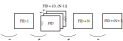
\includegraphics[scale=0.85]{algorithm}
    \caption{General case with $N \in \{1..(\text{BS}-2)\}$}
    \label{subfig:algorithm_general_case}
  \end{subfigure}
  \begin{subfigure}[b]{\textwidth}
    \includegraphics[scale=0.85]{algorithm_ex}
    \caption{Example with $N = 3$}
    \label{subfig:algorithm_example}
  \end{subfigure}
  \caption{Illustration of the image change detection algorithm}
  \label{fig:change_detection_algorithm}
\end{figure}

\begin{lstlisting}[style=C++]
  if (mean_diff >= threshold) {
      if (!throw_bgn) {
        throw_bgn_idx = frame_id;
        throw_bgn = true;
      }
  } else {
    if (throw_bgn) {
      throw_end_idx = frame_id;

      // Remove glitches (single frame changes)
      if ((throw_end_idx - throw_bgn_idx) == 1) {
        throw_bgn = false;
      } else {
        throw_end = true;
      }
    }
  }
\end{lstlisting}

% when no throw detected, release the Baumer buffer

\begin{lstlisting}[style=C++]
  if (!throw_bgn) {
    pBufferFilled->QueueBuffer();
  }
\end{lstlisting}
